\documentclass[a4paper,14pt]{extreport}
  \usepackage[left=1.5cm,right=1.5cm,
      top=1.5cm,bottom=2cm,bindingoffset=0cm]{geometry}
\usepackage[utf8]{inputenc}
\usepackage[english,ukrainian]{babel}
\usepackage{indentfirst}
\usepackage{misccorr}
\usepackage{graphicx}
\usepackage[dvipsnames]{xcolor}
\usepackage{cmap}

\usepackage{amsmath,amsfonts,amssymb,amsthm,mathtools}

\usepackage{icomma}
\usepackage{multirow}
\usepackage{geometry} 
\usepackage{euscript}
\usepackage{mathrsfs}
\usepackage{mathtext}
\usepackage{graphicx}
\usepackage{booktabs}
\usepackage{color}
\usepackage{rotating}
\usepackage{pdflscape}

\usepackage{subcaption}

\usepackage{calc}
\usepackage{hyperref}
\usepackage{floatrow}
\floatsetup[table]{capposition=top}
\usepackage{tikz}
\usepackage[siunitx]{circuitikz}
%\usetikzlibrary{er,positioning}
%\usetikzlibrary{positioning, fit, calc, er, shapes.geometric, arrows, decorations.markings}

\usetikzlibrary{shapes}
\usetikzlibrary{positioning,arrows}

%\usetikzlibrary{shapes.geometric, arrows}



\linespread{1.3}
\setlength{\parindent}{5ex}


\begin{document}

\pagecolor{white}
\begin{titlepage}
  \begin{center}
    \large
    Національний технічний університет України \\ "Київський політехнічний інститут імені Ігоря Сікорського"
     
       
    Факультет Електроніки
     
    Кафедра мікроелектроніки
    \vfill
      
    \textsc{ЗВІТ}\\
     
    {\Large Про виконання лабораторної роботи №5\\
      з дисципліни: «Фізичні основи сенсорики»\\[1cm]
      
     Сенсори освітленості\\
    
    }
  \bigskip
\end{center}
\vfill
 
\newlength{\ML}
\settowidth{\ML}{«\underline{\hspace{0.4cm}}» \underline{\hspace{2cm}}}
\hfill
\begin{minipage}{1\textwidth}
Виконав:\\
Студент 4-го курсу \hspace{4cm} $\underset{\text{(підпис)}}{\underline{\hspace{0.2\textwidth}}}$  \hspace{1cm}Мнацаканов А.С.\\
\vspace{1cm}

Перевірила: \hspace{6.1cm} $\underset{\text{(підпис)}}{\underline{\hspace{0.2\textwidth}}}$  \hspace{1 cm}Коваль В.М.\\

\end{minipage}

\vfill

\begin{center}
2021
\end{center}
\end{titlepage}





\begin{center}
\textbf{ Мета роботи}
\end{center}



Отримати практичні навички роботи з сенсорами
освітленності резистивного та діодного типу, здійснити їх калібрування та
визначити основні характеристики.


\begin{center}
\textbf{Короткі теоретичні відомості}
\end{center}

Датчик освітленості або сутінковий вимикач – це пристрій автоматичного
управління джерелом світла в залежності від рівня освітленості навколишнього
простору. Структура сутінкового вимикача досить проста і умовно може бути
розбита на три основні складові: фотоприймач (фотодіод, фоторезистор,
фототранзистор), пороговий пристрій (компаратор), вихідний пристрій (реле або
сімістор). Принцип роботи датчика освітленості полягає в тому, що при зміні
параметрів фотоелемента спрацьовує граничний пристрій (компаратор), який
подає сигнал на вихідний пристрій, що і включає освітлення. Наприклад, при
природному освітленні опір фоторезистора низький і напруга на ньому не
перевищує порогу спрацювання компаратора, тому штучне освітлення
відключене. Зменшення природного освітлення призводить до зростання опору
фоторезистора і відповідно напруги на ньому. В певний момент (за певного рівня
освітленності) рівень напруги на фоторезисторі досягає порогу спрацювання
компаратора, який за допомогою реле включає штучне освітлення.\\

Датчики освітленості встановлюються в місцях, де в денний час доби
простір освітлюється природним світлом, а при настанні темряви – штучним
світлом: для вуличного освітлення тротуарів, дворів житлових будинків, дитячих майданчиків; для освітлення автомагістралей; для контролю ілюмінації рекламних
щитів; для підсвічування вітрин тощо. Завдяки автоматичному спрацюванню
включення штучного джерела світла, з яким взаємодіє датчик освітлення,
споживання електрики зводиться до необхідного мінімуму.\\

Сучасні сутінкові вимикачі можуть бути обладнанні додатковими
датчиками, які значно розширюють робочі функції цих приладів (датчики руху,
таймери тощо). Наприклад, якщо разом з фотореле працює датчик руху, то
вуличний ліхтар включається в темний час доби за наявності в полі зору рухомих
об’єктів. Для уникнення автоматичного відключення вуличної реклами при світлі
автомобільних фар використовується так звана функція затримки вимкнення, яка
полягає в тому, що коли рівень освітлення зростає до рівня виключення, в
контролері активується відлік на встановлений термін, і якщо рівень освітлення з
часом не змінився, тоді фотореле вводиться в дію (штучне освітлення
вимикається). Фотореле з функцією таймера може вмикати/вимикати штучне
освітлення не тільки виходячи з рівня освітлення, але й в чітко визначений час.
Наприклад, підсвітка реклами автоматично відключається після півночі через її
неефективність в цей час доби).\\

Фотоприймачі, які використовуються в датчиках освітленості, працюють на
явищі внутрішнього фотоефекта і по суті здійснюють перетворення енергії
електромагнітного випромінювання в електричну енергію. Якщо енергія
падаючих фотонів є більшою, аніж ширина забороненої зони матеріалу, то в
результаті взаємодії фотонів з атомами речовини будуть вивільнятись носії
заряду, що можуть переміщатись всередині матеріалу під дією електричного поля
(явище внутрішнього фотоефекту). В фотоприймачах цей ефект проявляється у
вигляді зростання їх питомої провідності під час опромінення внаслідок
зростання кількості вільних носіїв заряду (фотоносіїв).\\

В якості фотоприймачів в датчиках освітленності використовуються
фоторезистори або фотодіоди. Фоторезистор – це напівпровідниковий резистор, принцип дії якого базується на зміні опору напівпровідника під дією світла. У
фоторезисторі за рахунок внутрішнього фотоефекту зростає кількість вільних
носіїв заряду, а тому електричний опір матеріалу приладу зменшується.
Залежність електричних властивостей фоторезистора від параметрів світлового
потоку виражається на світловій ВАХ. Фоторезистор характеризується
високою чутливістю, однак низькою швидкодією.\\

\begin{figure}[!h]\CenterFloatBoxes\TopFloatBoxes
 \ffigbox{\caption{Світлові та темнові ВАХ фоторезистора (а) та фотодіода (б)}}
{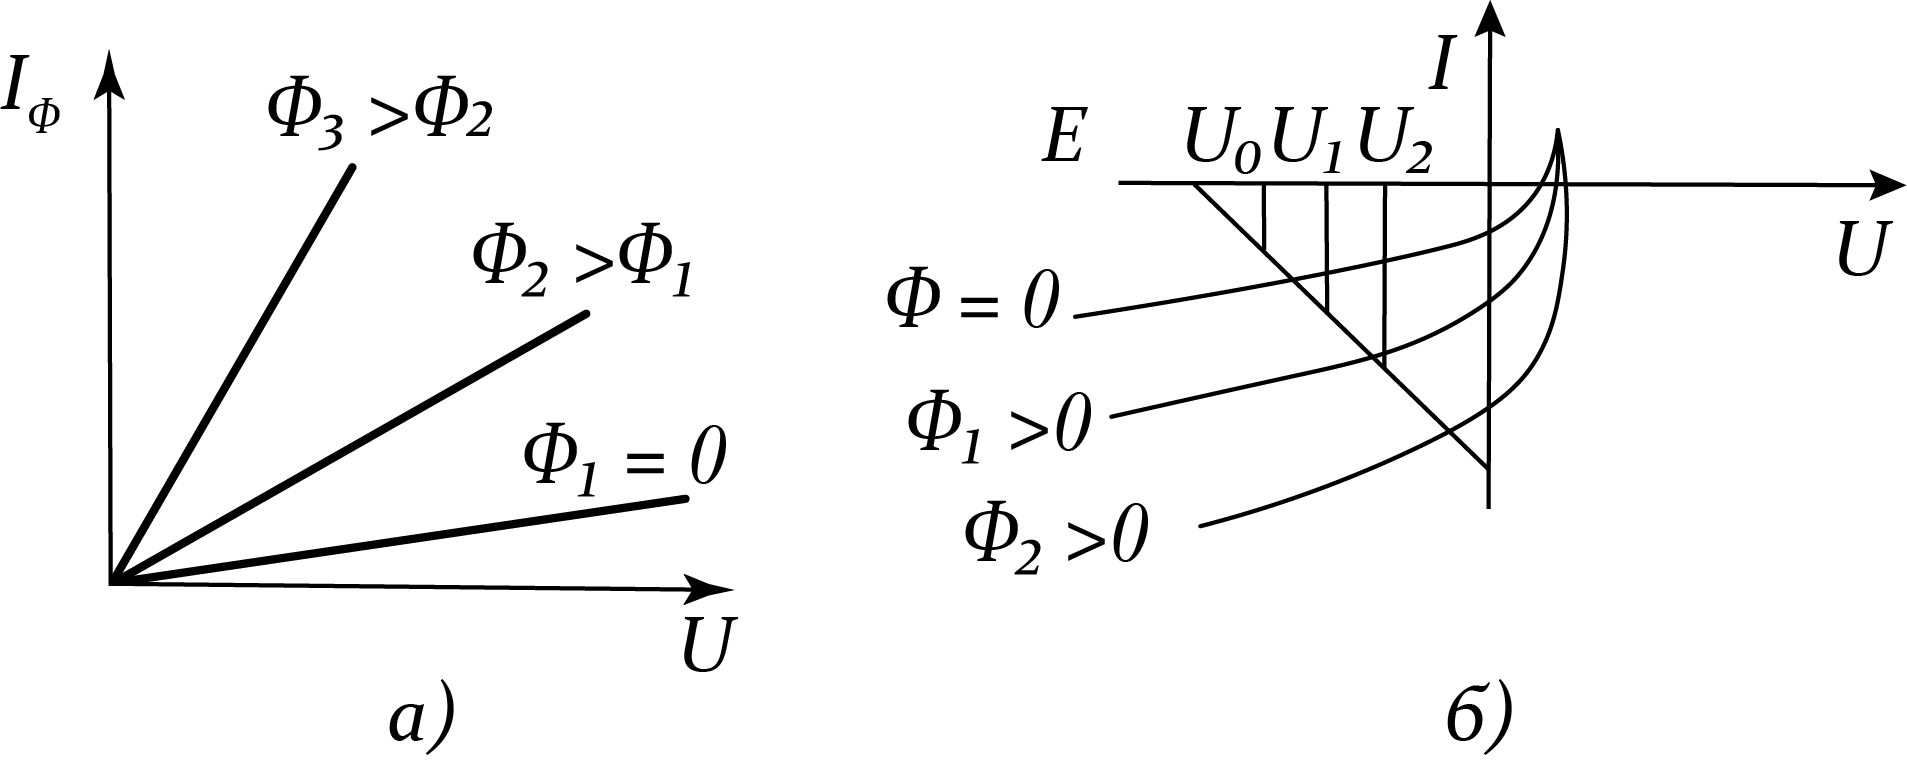
\includegraphics[scale=1]{11}}
\end{figure}

Фотодіод – це напівпровідниковий діод, принцип дії якого ґрунтується на
зміні зворотнього струму p-n-переходу в залежності від інтенсивності падаючого
світла. В результаті поглинання фотонів з енергією, більшою, аніж ширина
забороненої зони, в n-області з’являються електронно-діркові пари, які
розділяються електронним полем p–n-перехода наступним чином: дірки
переходять в р-область, а електрони залишаються в n-області. В результаті струм
через p–n-перехід викликаний дрейфом неосновних носіїв – дірок. Дрейфовий
струм фотоносіїв називають фотострумом, величина якого залежить від рівня
освітленості. На відміну від фоторезисторів фотодіоди характеризуються
вищою швидкодією.\\

Основним фоточутливим параметром фотоприймачів є коефіцієнт
фоточутливості, який визначається по люкс-амперній характеристиці (ЛАХ) за
формулою:

\begin{equation}
K_{\text{ф}}=\dfrac{I_{\text{ф}_2}-I_{\text{ф}_1}}{(\Phi_2-\Phi_1)\cdot U}=\dfrac{I_{\text{ф}_2}-I_{\text{ф}_1}}{(E_2-E_1)\cdot S\cdot U},
\end{equation}
де Kф – коефіцієнт фоточутливості, А/лмВ; $I_{\text{ф}}$ – фотострум; $\Phi$– світловий потік; E – освітленість; S – площа зразку; U – напруга, при якій проводились вимірювання ЛАХ.


\begin{center}
\textbf{Опис лабораторного стенду}
\end{center}

Лабораторний стенд для дослідження сенсорів освітленності складається з
наступних приладів:

\begin{trivlist}
\item 1) Люксметр цифровий LX1010BS;
\item 2) Освітлювач з предметним столиком та системою зондів на магнітах;
\item 3) Джерело постійного струму Б5-47;
\item 4) Мультиметр цифровий В7-35.
\end{trivlist}

Освітлювач складається з опорної плити, на якій розміщаються предметний
столик та система зондів на магнітах, а також вертикальний шток зі
шкалою в см і джерело світла.\\

Предметний столик призначений для розміщення лабораторних зразків і
вимірювання їх характеристик. Структура столика наступна:
алюмінієвий тепловідвід з посрібленою поверхнею (для електричного з’єднання з
тильним контактом лабораторного зразку), зачорнений екран (для вимірювання
темнових характеристик) та система магнітних зондів (притискні голчасті
контакти для електричного з’єднання з фронтальними контактами лабораторного
зразку). Максимальний розмір дослідних зразків становить 12$\times$17 мм.\\

Джерело світла закріплене на рухомій каретці вертикального
штоку і може переміщатись вздовж нього. Відстань від джерела світла до
предметного столику визначається по краю каретки на шкалі (відповідний рівень
позначений червоною крапкою, рис.). Діапазон переміщення освітлювача по
вертикалі до предметного столику становить 3...18 см.\\









Величина освітленості зразку вимірювалась за допомогою цифрового
люксометра LX1010BS. Порядок роботи з цим приладом наступний:

\begin{trivlist}
\item 1. Зняти пластикову кришку корпуса сенсора світла з написом “Open”.
\item 2. Ввімкнути прилад за допомогою перемикача “ON”.
\item 3. Розмістити сенсор світла на робочому столику і ввімкнути освітлювач.
\item 4. Встановити необхідний діапазон вимірювання освітленості за допомогою
перемикача діапазонів "2000 / 20 000 / 100 000" і користуючись табл.
встановити заданий рівень освітленості.
\item 5. Провести калібрування освітлювача, тобто виміряти величину
освітленості люксметром на різних рівнях розміщення джерела світла.
\item 6. Після завершення вимірювань закрити сенсор світла пластиковою
кришкою.
\item 7. Вимкнути люксометр за допомогою перемикача “OFF”.
\end{trivlist}


\begin{center}
\textbf{Порядок виконання роботи}
\end{center}


\begin{enumerate}
\item Ввімкнути вимірювальне обладнання лабораторного стенду.
\item Здійснити калібрування освітлювача.

\begin{trivlist}
\item 2.1. Виставити лампу за допомогою ручки на рухомому штативі на
максимальному рівні (18 см).
\item 2.2. Встановити люксметр на предметний столик. Для цього слід відкрутити
передню гайку і відвести в сторону столик для розміщення дослідних
зразків. Встановити чутливий елемент люксметра між двома гвинтами і
закріпити гумовим затискачем.
\item 2.3. З дисплею люксметра записати показ рівня освітленості поверхні
чутливого елементу за його максимальної відстані до освітлювача.
\item 2.4. Провести аналогічні вимірювання освітленості, знижуючи кожного разу
освітлювач на 2 поділки по штативу до мінімального рівня (4 см).
\item 2.5. Після завершення калібрування освітлювача предметний столик
повернути у вихідний стан.
\end{trivlist}

\item Провести вимірювання електричних характеристик сенсора освітленності резистивного типу.

\begin{trivlist}
\item 3.1. За допомогою пінцету встановити зразок сенсора освітленності на
предметний столик і закрити його темновим екраном.
\item 3.2. Розмістити зонди на магнітах на верхні контактні майданчики сенсора.
\item 3.3. Під’єднати зонди до вимірювального обладнання наступним чином:
зонд із зеленим маркуванням розмістити в роз’єм “+” на джерелі постійного
струму Б5-47, а зонд із синім маркуванням розмістити в роз’єм “ВХІД” на
мультиметрі цифровому В7-35, вільним провідником з’єднати джерело
постійного струму та мультиметр між собою.
\item 3.4. Провести вимірювання струму, що протікає крізь сенсор, в діапазоні
напруг від 0,5 до 6,5 В з кроком 0,5 В.
\item 3.5. Змінити полярність прикладеної напруги шляхом зміни провідників
місцями на джерелі постійного струму Б5-47.
\item 3.6. Провести вимірювання струму, що протікає крізь сенсор, в діапазоні
напруг від 0,5 до 6,5 В з кроком 0,5 В.
\end{trivlist}

\item Провести вимірювання фоточутливої характеристики (люкс-амперної характистики (ЛАХ)) сенсора освітленності резистивного типу.

\begin{trivlist}
\item 4.1. Зняти із зразку сенсора освітленності темновий екран.
\item 4.2. Ввімкнути освітлювач та виставити його на максильно високому рівні за
допомогою рухомої ручки на штативі (18 см).
\item 4.3. Виставити на джерелі постійного струму Б5-47 зворотню напругу 6,5 В.
\item 4.4. Виміряти за допомогою мультиметра цифрового В7-35 світловий струм
сенсора.
\item 4.5.Провести аналогічні вимірювання світлового струму сенсора, знижуючи
кожного разу освітлювач на 2 поділки по штативу до мінімального рівня (4 см).
\end{trivlist}

\item Провести вимірювання електричних характеристик сенсора освітленності діодного типу.

\begin{trivlist}
\item 5.1. За допомогою пінцету встановити зразок сенсора освітленності на
предметний столик і закрити його темновим екраном.
\item 5.2. Розмістити зонд із зеленим маркуванням на верхній контактний
майданчик сенсора (лівий або правий), а синій зонд для даного типу
вимірювань не задіяний. Натомість для вимірювання ВАХ фотодіоду слід
використати провідник з червоним маркуванням, що являє собою нижній
контакт p-n-переходу.
\item 5.3. Під’єднати зонди до вимірювального обладнання наступним чином:
зонд із зеленим маркуванням розмістити в роз’єм “+” на джерелі постійного
струму Б5-47, а зонд із червоним маркуванням розмістити в роз’єм “ВХІД”
на мультиметрі цифровому В7-35, вільним провідником з’єднати джерело
постійного струму та мультиметр між собою.
\item 5.4. Провести вимірювання струму, що протікає крізь сенсор, в діапазоні
напруг від 0,5 до 6,5 В з кроком 0,5 В.
\item 5.5. Змінити полярність прикладеної напруги шляхом зміни провідників
місцями на джерелі постійного струму Б5-47.
\item 5.6. Провести вимірювання струму, що протікає крізь сенсор, в діапазоні
напруг від 0,5 до 6,5 В з кроком 0,5 В.
\end{trivlist}


\item Провести вимірювання фоточутливої характеристики (люкс-амперної характистики (ЛАХ)) сенсора освітленності діодного типу.

\begin{trivlist}
\item 6.1. Зняти із зразку сенсора освітленності темновий екран.
\item 6.2. Ввімкнути освітлювач та виставити його на максильно високому рівні за допомогою рухомої ручки на штативі (18 см).
\item 6.3. Виставити на джерелі постійного струму Б5-47 зворотню напругу 6,5 В.
\item 6.4. Виміряти за допомогою мультиметра цифрового В7-35 світловий струм сенсора.
\item 6.5.Провести аналогічні вимірювання світлового струму сенсора, знижуючи
кожного разу освітлювач на 2 поділки по штативу до мінімального рівня (4 см).
\end{trivlist}

\item Вимкнути вимірювальне обладнання.

\end{enumerate}
\begin{center}
\textbf{Обробка результатів роботи}
\end{center}

\begin{trivlist}
\item 1. Скласти таблицю для калібрування освітлювача, за якою можна встановити
рівень освітленості поверхні в залежності від місцезнаходження
освітлювача.
\item 2. Побудувати ВАХ сенсорів освітленості резистивного та діодного типу.
Розрахувати їх коефіцієнти випрямлення за напруги 6,5 В як відношення
прямого струму до зворотнього. У висновку порівняти ВАХ обох сенсорів.
\item 3. Скласти таблиці для калібрування сенсорів освітленості резистивного та
діодного типу
\item 4. Побудувати ЛАХ сенсорів освітленості резистивного та діодного типу. У
висновку порівняти два типи сенсорів за чутливістю.
\end{trivlist}
\newpage

\begin{center}
\textbf{Результати вимірювань}
\end{center}


\begin{table}[!h]
    \caption{ВАХ сенсорів освітленості}
    \begin{subtable}{.5\linewidth}
      \centering
     \caption{резистивного типу}
\begin{tabular}{|c|c|c|c|}
\hline
\multicolumn{2}{|c|}{Пряма} & \multicolumn{2}{c|}{Зворотня} \\ \hline
U, В        & І, мкА        & U, В         & І, мкА         \\ \hline
0,5         & 0,9           & 0,5          & 0,9            \\ \hline
1           & 1,2           & 1            & 1,3            \\ \hline
1,5         & 1,5           & 1,5          & 1,5            \\ \hline
2           & 1,7           & 2            & 1,7            \\ \hline
2,5         & 1,8           & 2,5          & 1,8            \\ \hline
3           & 2             & 3            & 1,9            \\ \hline
3,5         & 2,1           & 3,5          & 2              \\ \hline
4           & 2,3           & 4            & 2,1            \\ \hline
4,5         & 2,4           & 4,5          & 2,1            \\ \hline
5           & 2,5           & 5            & 2,2            \\ \hline
5,5         & 2,7           & 5,5          & 2,3            \\ \hline
6           & 2,8           & 6            & 2,3            \\ \hline
6,5         & 2,9           & 6,5          & 2,4            \\ \hline
\end{tabular}
\end{subtable}%
\begin{subtable}{.5\linewidth}
\centering
 \caption{діодного типу}
\begin{tabular}{|c|c|c|c|}
\hline
\multicolumn{2}{|c|}{Пряма} & \multicolumn{2}{c|}{Зворотня} \\ \hline
U, В        & І, мкА        & U, В         & І, мкА         \\ \hline
0,5         & 16,9          & 0,5          & 0,8            \\ \hline
1           & 50            & 1            & 1,2            \\ \hline
1,5         & 87,3          & 1,5          & 1,5            \\ \hline
2           & 127,9         & 2            & 1,7            \\ \hline
2,5         & 171           & 2,5          & 1,8            \\ \hline
3           & 205           & 3            & 2              \\ \hline
3,5         & 228           & 3,5          & 2,1            \\ \hline
4           & 250           & 4            & 2,3            \\ \hline
4,5         & 266           & 4,5          & 2,4            \\ \hline
5           & 273           & 5            & 2,6            \\ \hline
5,5         & 309           & 5,5          & 2,7            \\ \hline
6           & 347           & 6            & 2,9            \\ \hline
6,5         & 383           & 6,5          & 3              \\ \hline
\end{tabular}
\end{subtable} 

\end{table}


\begin{table}[!h]
    \caption{ЛАХ сенсорів освітленості}
    \begin{subtable}{.5\linewidth}
      \centering
     \caption{резистивного типу}
\begin{tabular}{|c|c|}
\hline
$E_{\upsilon}$, лк & І, мкА \\ \hline
7500               & 47,5   \\ \hline
8500               & 52,6   \\ \hline
9900               & 58,7   \\ \hline
11700              & 66,7   \\ \hline
13600              & 75,9   \\ \hline
15700              & 86,3   \\ \hline
18500              & 96,7   \\ \hline
22100              & 110,7  \\ \hline
\end{tabular}
\end{subtable}%
\begin{subtable}{.5\linewidth}
\centering
 \caption{діодного типу}
\begin{tabular}{|c|c|}
\hline
$E_{\upsilon}$, лк & І, мкА \\ \hline
7500               & 46,3   \\ \hline
8500               & 51,4   \\ \hline
9900               & 57,4   \\ \hline
11700              & 64,7   \\ \hline
13600              & 72,7   \\ \hline
15700              & 82,7   \\ \hline
18500              & 92,3   \\ \hline
22100              & 105,6  \\ \hline
\end{tabular}
\end{subtable} 

\end{table}



\begin{center}
\textbf{Графіки}
\end{center}




\begin{figure}[!h]\CenterFloatBoxes\TopFloatBoxes
 \ffigbox{\caption{Темнова ВАХ сенсора освітленості резистивного типу}\label{darkres}}
{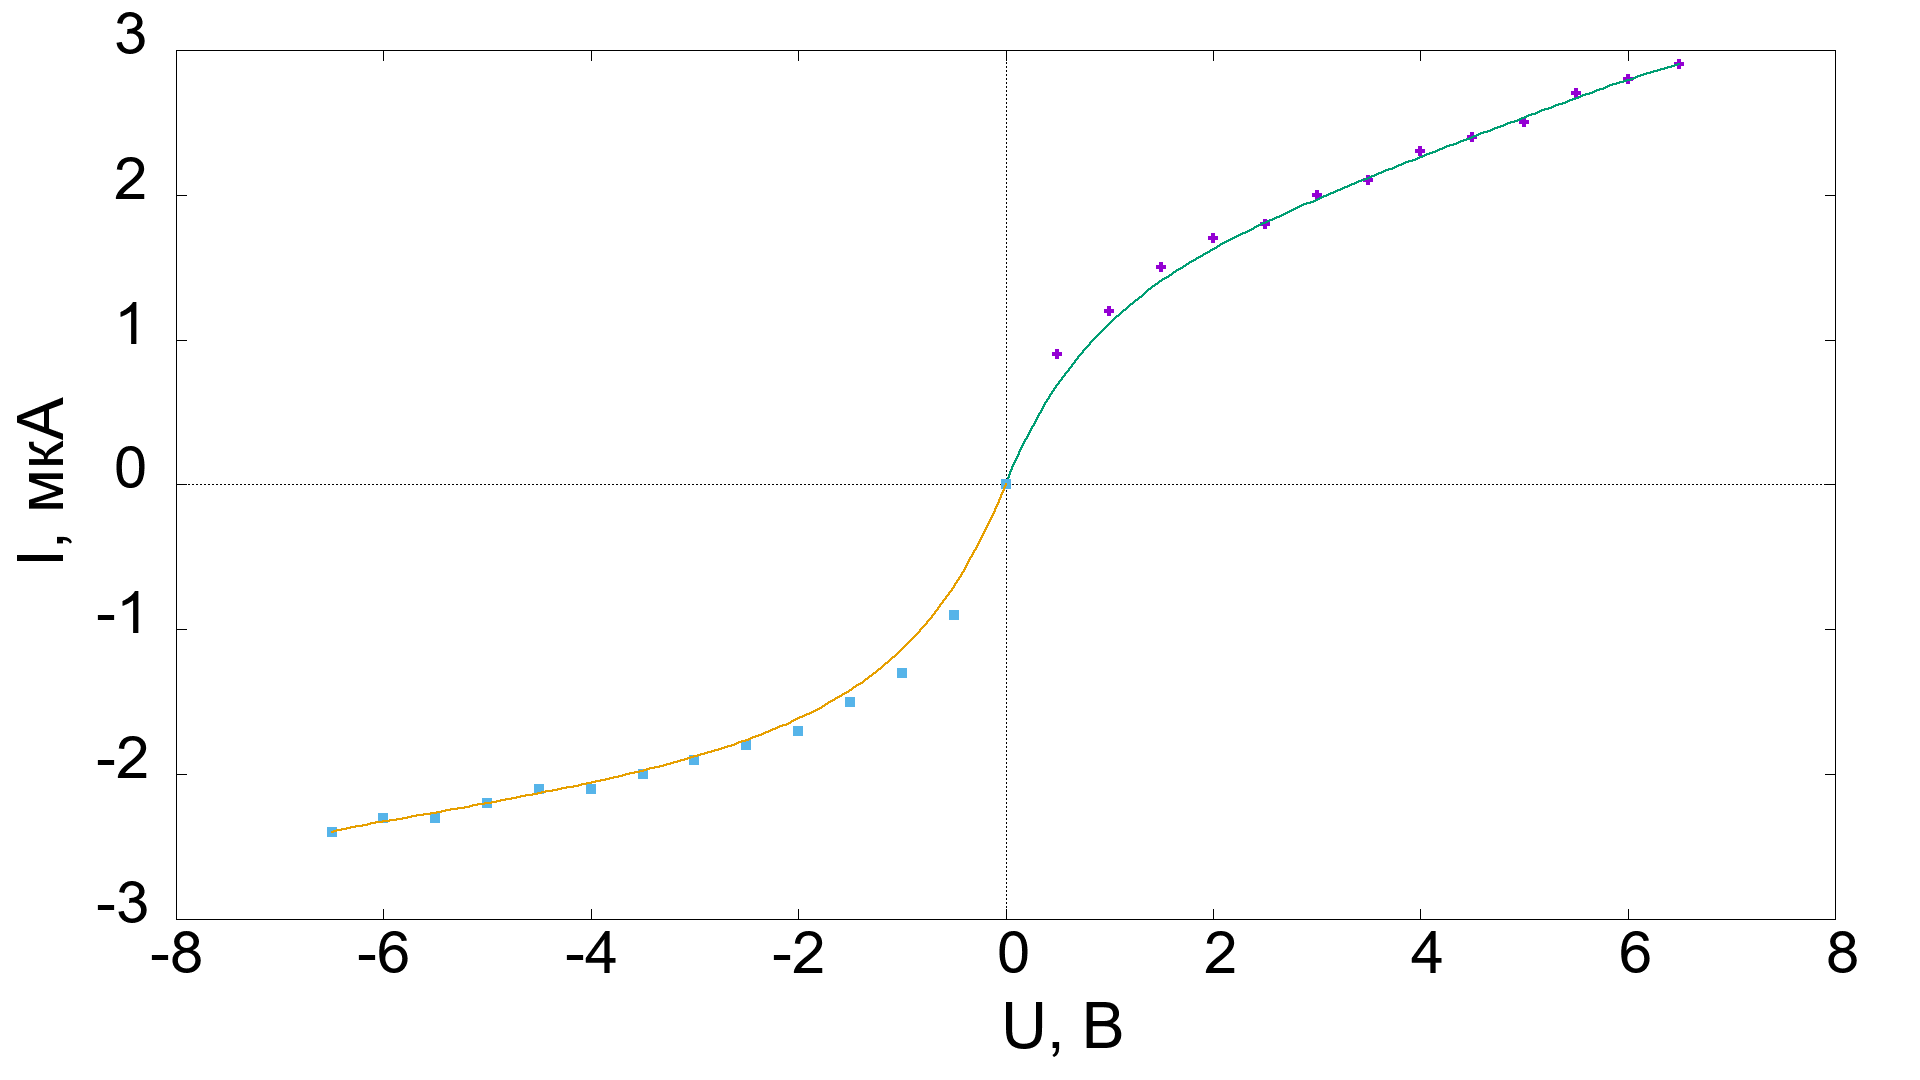
\includegraphics[scale=0.3]{tr.png}}
\end{figure}

\begin{figure}[!h]\CenterFloatBoxes\TopFloatBoxes
 \ffigbox{\caption{Темнова ВАХ сенсора освітленості діодного типу}\label{darkdio}}
{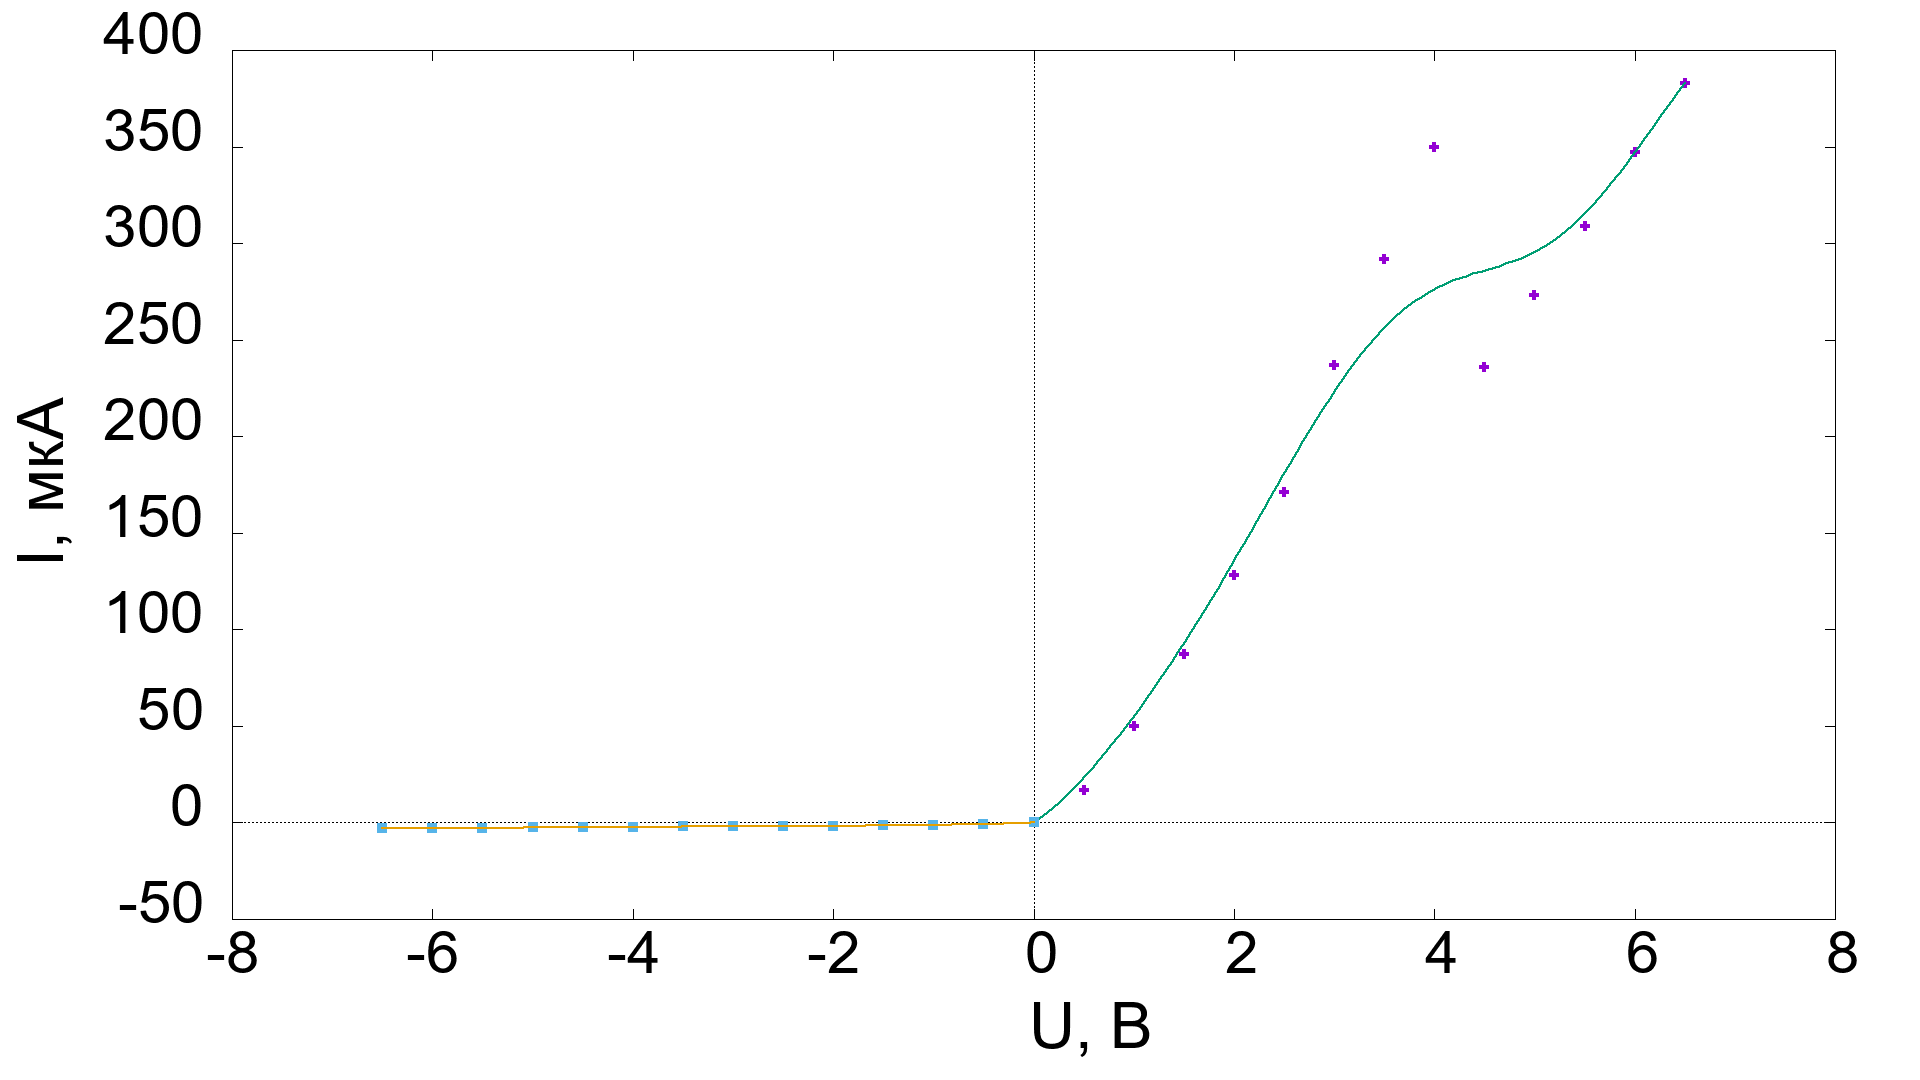
\includegraphics[scale=0.3]{td.png}}
\end{figure}

\newpage

\begin{figure}[!h]\CenterFloatBoxes\TopFloatBoxes
 \ffigbox{\caption{ЛАХ сенсорів освітленості}}
{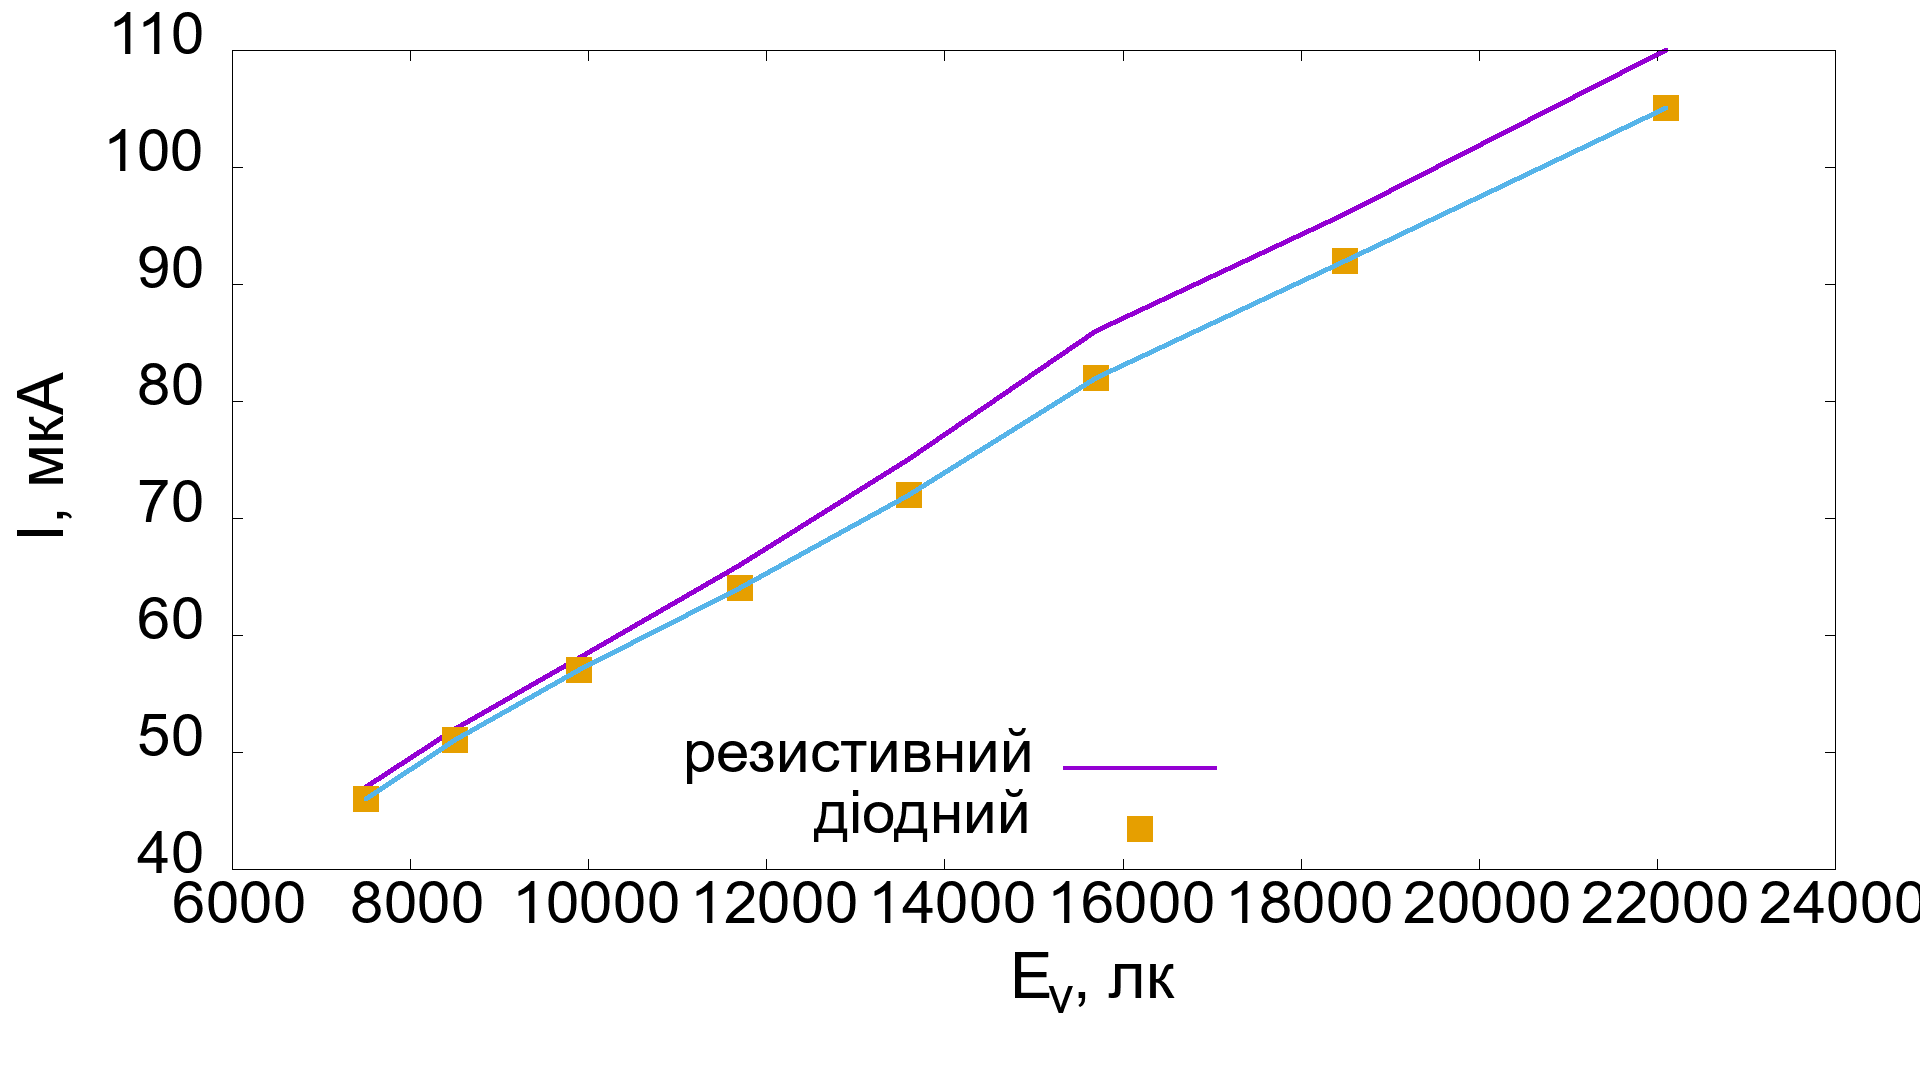
\includegraphics[scale=0.3]{lax.png}\label{luxx}}
\end{figure}


\begin{center}
\textbf{Висновок}
\end{center}



Проаналізувавши ВАХ сенсорів освітленості, бачимо, що сенсор резистивного типу (рис.\ref{darkres}) має більш лінійну залежність ніж сенсор діодного типу (рис.\ref{darkdio}). Сенор діодного типу має характерну для більшості діодів круту експоненціальну залежність, тобто при невеликих збільшень напруги струм зростає на порядок чи навіть на два, відбуваєтся більш стрімка зміна опору $\Rightarrow$ сенсор діодного типу швидший ніж резистивний, але на ЛАХ(рис.\ref{luxx}) нахил кривої сенсора резистивного типу крутіший, ніж у сенсора діодного типу $\Rightarrow$   фоточутливість сенсора освітленості резистивного типу вища ніж у діодного.


\newpage
\begin{center}
\textbf{Контрольні запитання}
\end{center}


\begin{trivlist}
\item 1. Що собою являє датчик освітленості? Яка його структура?
\item 2. В чому полягає принцип дії сутінкового вимикача? Наведіть приклади.
\item 3. Перелічіть області використання датчика освітленості. Які переваги забезпечує застосування даного типу датчика?
\item 4. Вкажіть на додаткові датчики, які можуть використовуватись у складі сутінкових вимикачів. Яким чином вони розширюють базові функції цих приладів?
\item 5. В чому полягає явище внутрішнього фотоефекту? Яким чином дане явище проявляється у фотоприймачах?
\item 6. Які види фотоприймачів використовуються в датчиках освітленності? Порівняйте їх між собою за основними характеристиками.
\item 7. Назвіть принцип дії фоторезисторів та перелічіть їх основні параметри і характеристики.
\item 8. Назвіть принцип дії фотодіодів та перелічіть їх основні параметри і характеристики.
\end{trivlist}






\end{document}